\documentclass{article}

% if you need to pass options to natbib, use, e.g.:
\PassOptionsToPackage{numbers, compress}{natbib}
% before loading nips_2017
%
% to avoid loading the natbib package, add option nonatbib:
% \usepackage[nonatbib]{nips_2017}

%\usepackage{nips_2017}
\usepackage[final]{nips_2017}
\bibliographystyle{abbrvnat}

% to compile a camera-ready version, add the [final] option, e.g.:
%\usepackage[final]{nips_2017}

\usepackage[utf8]{inputenc} % allow utf-8 input
\usepackage[T1]{fontenc}    % use 8-bit T1 fonts
\usepackage{hyperref}       % hyperlinks
\usepackage{url}            % simple URL typesetting
\usepackage{booktabs}       % professional-quality tables
\usepackage{amsfonts}       % blackboard math symbols
\usepackage{nicefrac}       % compact symbols for 1/2, etc.
\usepackage{microtype}      % microtypography
\usepackage{amsmath}
\usepackage{algorithm}
\usepackage{algpseudocode}
\usepackage{graphicx}

\providecommand{\scan}{\text{SCAN}}
\providecommand{\reduce}{\text{REDUCE}}
% declaration of the new block
\algblock{ParFor}{EndParFor}
% customising the new block
\algnewcommand\algorithmicparfor{\textbf{parfor}}
\algnewcommand\algorithmicpardo{\textbf{do}}
\algnewcommand\algorithmicendparfor{\textbf{end\ parfor}}
\algrenewtext{ParFor}[1]{\algorithmicparfor\ #1\ \algorithmicpardo}
\algrenewtext{EndParFor}{\algorithmicendparfor}

\title{Parallelizing Linear Recurrent Neural Nets Over Sequence Length}

% The \author macro works with any number of authors. There are two
% commands used to separate the names and addresses of multiple
% authors: \And and \AND.
%
% Using \And between authors leaves it to LaTeX to determine where to
% break the lines. Using \AND forces a line break at that point. So,
% if LaTeX puts 3 of 4 authors names on the first line, and the last
% on the second line, try using \AND instead of \And before the third
% author name.

\author{
  Eric Martin \\%\thanks{Use footnote for providing further
    %information about author (webpage, alternative
    %address)---\emph{not} for acknowledging funding agencies.} \\
  %Some Affiliation\\
  \texttt{eric@ericmart.in}
  %% examples of more authors
  \And
  Chris Cundy \\
  \texttt{c.cundy@berkeley.edu}
  %%\texttt{some@email.com}
  %% Affiliation \\
  %% Address \\
  %% \texttt{email} \\
  %% \AND
  %% Coauthor \\
  %% Affiliation \\
  %% Address \\
  %% \texttt{email} \\
  %% \And
  %% Coauthor \\
  %% Affiliation \\
  %% Address \\
  %% \texttt{email} \\
  %% \And
  %% Coauthor \\
  %% Affiliation \\
  %% Address \\
  %% \texttt{email} \\
}

\begin{document}
% \nipsfinalcopy is no longer used

\maketitle

\begin{abstract}
Recurrent neural networks (RNNs) are widely used to model sequential data 
but their non-linear dependencies between sequence elements prevent parallelizing
training over sequence length. We show the training of RNNs with only 
linear sequential dependencies can be parallelized over the
sequence length using the parallel scan algorithm, leading to rapid training
on long sequences with small minibatch size. We abstract prior linear sequence models
into a new framework of linear surrogate RNNs and develop
a linear surrogate long short-term memory (LS-LSTM) powered by a parallel linear recurrence
CUDA kernel we implemented.
We evaluate the LS-LSTM on a long sequence noisy autoregressive task and find
the LS-LSTM achieves slightly superior train and test performance to a similar 
sized LSTM in 4x less training time. We analyze latency and throughput of
the LS-LSTM and find the LS-LSTM reaches up to 
175x the throughput of the LSTM in the small minibatch long sequence regime.
\end{abstract}

\section{Introduction}

Recurrent neural networks (RNNs) are widely used for sequence modelling tasks in domains such as 
natural language processing \cite{sutskever2014sequence}, 
speech recognition \cite{amodei2015deep},
and reinforcement learning \cite{hausknecht2015deep}. Most RNNs, including popular variants such as long short-term memories (LSTMs) \cite{hochreiter1997long} and gated recurrent units (GRUs) \cite{cho2014learning}, contain a non-linear dependency
between sequential inputs. These non-linear dependencies create a very flexible class of
models but limit the feasibility of training RNNs on long sequences as each sequence element
must be processed sequentially.
Modelling sequences of thousands to millions of elements is important to domains
such as robotics, remote sensing, control systems, speech recognition, medicine, and finance.

The RNN serial evaluation inefficiency problem is usually mitigated by parallelizing the forward
and backward pass over a minibatch of inputs. Without minibatches, RNN evaluation is a sequence of matrix-vector multiplications. Minibatches transform RNN computation into a sequence of more efficient matrix-matrix multiplications, but minibatches within RNNs present many issues.
RNN model size is often limited by GPU memory size, and running a forward 
and backward pass on a minibatch requires memory linear in
the minibatch size.
Grouping data into minibatches increases the latency of each pass and reduces the rate of optimization steps. Finally, training with larger minibatches damages generalization ability 
\cite{keskar2017large}. Persistent RNNs \cite{diamos2016persistent} use a novel implementation that can achieve high GPU utilization with very small 
minibatch sizes when the recurrent state is larger than 500 elements, but even
persistent RNNs become limited by the serial evaluation
inefficiency at smaller hidden sizes.

Numerous prior works have shown strong performance from neural sequential models with only linear dependence on earlier sequence elements. \citet{balduzzi2016strongly} investigated RNNs with only elementwise linear recurrence relations 
$h_t = \alpha_t \odot h_{t-1} + (1-\alpha_t) \odot x_t$ and developed
linear variants of LSTM and GRU that perform similarly to
standard non-linear RNNs on text generation tasks. \citet{bradbury2017quasi},  \citet{kalchbrenner2016neural}, \citet{gehring2017convolutional}, and \citet{van2016wavenet} have successfully applied networks of convolutions over sequences for tasks
such as machine translation, language modelling, and audio generation. 
These works have observed up to an order of magnitude 
increase in training throughput compared to RNN alternatives. Convolutional sequence models typically rely on either an attention mechanism or a (possibly linear) recurrent layer
to integrate information at scales larger than the filter width. Introduction of a recurrent
layer prevents full parallelization over the sequence length while attention mechanisms are
expensive to apply on long sequences in online inference use cases.
One dimensional convolution can be viewed as a learnable linear
finite impulse response (FIR) filter with a parallel evaluation algorithm, while
linear recurrence is a learnable linear infinite impulse response (IIR). This work
parallelizes evaluation of linear recurrences through application of the parallel
scan algorithm.

Scans and reductions are computations involving repeated application of a binary
operator $\oplus$ over an array of data. Computing the sum or maximum
of an array is an example of a reduction, while a cumulative sum is a common
example of a scan operation. Throughout this work, the scan of $\oplus$ with
initial value $b$ is defined as
\begin{align*}
\scan(\oplus, [a_1, a_2, ..., a_n], b) = [(a_1 \oplus b), (a_2 \oplus a_1 \oplus b), ..., (a_n \oplus a_{n-1} ... \oplus a_1 \oplus b)]
\end{align*}
The reduction of $\oplus$ over array $A$ and initial value $b$ is denoted 
$\reduce(\oplus, A, b)$ and is the final element of $\scan(\oplus, A, b)$.
Despite their dependent computation graph, algorithms exist to parallelize scans 
and reductions when $\oplus$ is associative \cite{ladner1980parallel}.

\citet{blelloch1990prefix} shows that first order recurrences of the form
$h_t = (\Lambda_t \otimes h_{t-1}) \oplus x_t$ can be parallelized with
the parallel scan algorithm if three conditions are met:

\begin{enumerate}
\item $\oplus$ is associative: $(a \oplus b) \oplus c = a \oplus (b \oplus c)$
\item $\otimes$ is semiassociative: there exists a binary associative operator
$\odot$ such that $a \otimes (b \otimes c) = (a \odot b) \otimes c$
\item $\otimes$ distributes over $\oplus$: $a\otimes(b\oplus c) = (a\otimes b) \oplus (a \otimes c)$ 
\end{enumerate}

Our primary contribution is the application of the parallel linear recurrence algorithm to RNNs.

\section{Parallel linear recurrence}

Using elementwise vector addition as $x \oplus y= x+y$, matrix-vector multiplication as $A \otimes x=Ax$,
and matrix-matrix multiplication as $A \odot B=AB$ satisfies Blelloch's three conditions, thus allowing linear
recurrence $h_t = \Lambda_t h_{t-1} + x_t$ to be evaluated in parallel over $t$ for
vectors $x_t$ and square matrices $\Lambda_t$. As the method is
essential to this work, Algorithm 1 presents the parallel linear recurrence algorithm
for the interested reader.
\begin{algorithm}
\caption{Parallel linear recurrence on $p$ processors}
\begin{algorithmic}[1]
  \State Let $y = [(\Lambda_1, x_1), (\Lambda_2, x_2), ..., (\Lambda_T, x_T)]$
  \State Let binary operator $\bullet$ act as $(\Lambda, x) \bullet h = \Lambda h + x$
  \State Let $S_0=1, S_i < E_i, E_i + 1 = S_{i+1}, E_{p-1}=T$ for $i$ in $0,p-1$

  \\
  \ParFor{$i \gets 0,p-1$}
    \State $P_i = \reduce(\odot, \Lambda_{S_i:E_i}, I)$
    \State $R_i = \reduce(\bullet, y_{S_i:E_i}, 0)$
  \EndParFor

  \\
  \State Let $z = [(P_0, R_0), (P_1, R_1), ..., (P_p, R_p)]$.
  \State $C = \scan(\bullet, z, h_0)$   \Comment{compute $C_i = P_i C_{i-1} + R_i$ with $C_{-1}=h_0$}

  \\
  \ParFor{$i \gets 0,p-1$}
    \State $h_{S_i:E_i} = \scan(\bullet, y_{S_i:E_i}, C_{i-1})$
  \EndParFor
  
  \State \Return $h$
\end{algorithmic}
\end{algorithm}

\subsection{Theoretical performance}
The cost of a serial scan over a sequence of length $T$ is 
$C_\text{sscan} = (C_\otimes + C_\oplus)T$, compared to the parallel scan cost
$C_\text{pscan} = 2(C_\odot + C_\otimes + C_\oplus)(T/p + \lg p)$ \cite{blelloch1990prefix}.
If $h_t$ is a vector of dimension $n$ then 
$C_\odot=n^3, C_\otimes=n^2, C_\oplus=n$ giving
$C_\text{pscan} = 2(n^3 + n^2 + n)(T/p + \lg p)$ and 
$C_\text{sscan} = (n^2 + n)T$. The $n^3$ cost of the matrix
multiplication in the parallel algorithm can destroy any parallel speedups for
sufficiently large hidden states and lead to a slower algorithm overall.

To avoid this problem, we will only consider diagonal matrices $\Lambda_t$, in which
case matrix-matrix and matrix-vector have cost $n$ and 
$C_\text{pscan}=6n(T/p + \lg p)$ and $C_\text{sscan}=2nT$. Assuming $p \ll T$, then 
$C_\text{pscan} \le C_\text{sscan}$ when $p \ge 3$.
As we are only considering diagonal matrices, the
linear recurrence will be written $h_t = \lambda_t \odot h_{t-1} + x_t$ where
$\odot$ indicates elementwise multiplication.

Limiting $\Lambda_t$ to be diagonal may seem like a severe constraint but there are
several reasons to do so beyond the unfavorable parallelization performance. Relatively few neural
network models use separate recurrent matrices for each sequence element and using these
separate matrices would require potentially prohibitive $n^2T$ memory. Applying
the same matrix $\Lambda$ to each sequence element is also unappealing considering that a matrix
multiplication can be thought of as a rotation and a scaling. The same rotation at every
element seems unlikely to be useful, and the scaling is exactly what's captured in diagonal
vectors $\lambda_t$. Recurrent coefficient vectors $\lambda_t$ provide enough flexibility
to implement schemes such as exponential moving averages or a gating mechanism.

\subsection{Backpropagation}
\begin{align*}
\nabla_{h_T}L &= \frac{\partial L}{\partial h_T} \\
\nabla_{h_t}L &= \frac{\partial h_{t+1}}{\partial h_t} \odot \nabla_{h_{t+1}} L + \frac{\partial L}{\partial h_t} \\ 
&= \lambda_{t+1} \odot \nabla_{h_{t+1}} L + \frac{\partial L}{\partial h_t} \\
\nabla_{\lambda_t}L &= \frac{\partial h_t}{\partial\lambda_t} \odot \nabla_{h_t}L = h_{t-1} \odot \nabla_{h_t}L \\
\nabla_{x_t}L &= \nabla_{h_t} L \\
\nabla_{h_0}L &=  \frac{\partial h_1}{\partial h_0} \odot \nabla_{h_1} L = \lambda_1 \odot \nabla_{h_1} L
\end{align*}

The backpropagation equations center around a linear recurrence over $\frac{\partial L}{\partial h_t}$ in the reverse order of the original sequence. This allows for parallelizing both the forwards and backwards pass of a linear RNN over the sequence length.

\subsection{Implementation}
A modern high-end NVIDIA GPU consists of between 640 and 3200 concurrently
executing warps. Each warp operates on 32 single precision floating point numbers
in parallel.

This work implemented parallel linear recurrence as a CUDA kernel with
bindings into the TensorFlow \cite{abadi2016tensorflow} framework. Each warp acts as a processor, which means algorithmic $p$ is up to 3200 and the theoretical parallelization speedup factor is up to several hundred.
The 32 lanes of each warp work on different
elements of the recurrence vector in parallel. These implementation details mean that
peak performance is only obtained on sequences of at least several thousand
steps on at least a 32 element vector.

\section{Models}
Parallel linear recurrence can be used to construct a wide variety of differentiable modules that can be evaluated in parallel. Common applications of linear recurrence include gating schemes and exponential moving averages. Although linear recurrence values can depend only linearly on previous elements, the stacking of linear recurrent layers separated by non-linearities allows for a non-linear dependence on the past. In this sense the non-linear depth of a linear recurrent network is the number of layers and not the sequence length. 

\subsection{Gated impulse linear recurrent layer}
A gated impulse linear recurrent (GILR) layer transforms its $m$ dimensional inputs $x_t$ into a sequence of $n$ dimensional hidden states $h_t$:
\begin{align*}
g_t &= \sigma(Ux_t + b_g) \\
i_t &= \tau(Vx_t + b_z) \\
h_t &= g_t \odot h_{t-1} + (1-g_t)\odot i_t
\end{align*}
A GILR layer applies the same non-linear transform to each sequence element and then accumulates the sequence elements with a non-linear gating mechanism. Gate $g_t$ uses the sigmoid activation function to have values in [0,1] for reasonable gating semantics, while impulse $i_t$ can use any activation function $\tau$. Stacking GILR layers allows for rich non-linear dependence on previous events while still taking advantage of fast parallel sequence evaluation.

\subsubsection{Impact on effective "batch size"}
Consider evaluating a vanilla RNN $h_t = \sigma(Uh_{t-1} + Vx_t + b)$ from $m$ inputs to $n$ hidden units on a sequence of length $T$ with minibatch size $b$ using a  serial evaluation strategy. At each of $T$ iterations, the naive approach performs two $(b, m) \mathbf{x} (m, n)$ matrix multiplications. Larger matrix multiplications achieve higher throughput due to less IO overhead, so the better approach computes $Vx_t$ for all $t$ ahead of time in a single $(bT, m) \mathbf{x} (m, n)$ matrix multiply. The non-linear recurrence forces even the better approach to perform $T$ potentially small $(b, m) \mathbf{x} (m, n)$ matrix multiplications in serial which makes performance heavily dependent on minibatch size.

Now consider the GILR, noting that it has the same two matrix-vector multiplications per iteration as the vanilla RNN. $g$ and $i$ can each be evaluated for all $t$ with a single $(bT, m) \mathbf{x} (m, n)$ matrix multiplication each. Given $g$ and $i$, $h$ can be computed using a parallel linear recurrence over $T$ vectors each of $bn$ elements. Rather than $T$ small operations, the GILR can be evaluated over all sequence elements with two large matrix multiplies and a parallel linear recurrence. GILR performance is much less dependent on batch size as the matrix multiplies see an "effective batch size" of $bT$ and $T$ is typically large.

\subsection{Linear surrogate RNNs}
RNNs learn a transition function $s_t = f(s_{t-1}, x_t)$ which combines previous state $s_{t-1}$ with input $x_t$ to compute current state $s_t$. Non-linear $f$ prevents application of the parallel linear recurrence algorithm and forces slow serial evaluation. To work around this inefficiency, note that $s_t$ serves a dual purpose. In $s_t = f(s_{t-1}, x_t)$, $s_{t-1}$ serves as an input to $f$ summarizing the previous inputs while $s_t$ serves as the output of $f$ to be passed to other layers of the network. If we decouple these uses, we can instead compute $s_t = f(\tilde{s}_{t-1}, x_t)$ with $\tilde{s}_t$ as a linearly computable surrogate for $s_t$. With this linear surrogate, non-linear $f$ can still be evaluated. We refer to this class of model as a linear surrogate RNN (LS-RNN). Quasi-RNNs \cite{bradbury2017quasi} are LS-RNNs using $\tilde{h}_{t-1} = W_k x_{t-k} + ... W_1 x_{t-1}$
and strongly typed RNNs\cite{balduzzi2016strongly} are LS-RNNs with $\tilde{h}_t=x_{t-1}$. Although not a rule, LS-RNNs can often be parallelized over sequence length with either
convolution or linear recurrence.

As an example LS-RNN, consider an LSTM:
\begin{align*}
f_t, i_t, o_t &= \sigma(U_{f,i,o} h_{t-1} + V_{f,i,o} x_t + b_{f,i,o}) \\
z_t &= \tau(U_z h_{t-1} + V_z x_t + b_z) \\
c_t &= f_t \odot c_{t-1} + i_t \odot z_t \\
h_t &= o_t \odot c_t
\end{align*}
An LSTM has state $s_t = (h_t, c_t)$. $c_t$ depends only linearly on $c_{t-1}$, so no surrogate is needed for $c_t$. $h_t$ has a non-linear dependence on $h_{t-1}$, so $h_t$ needs a linear surrogate. With a GILR layer as surrogate, the linear surrogate LSTM (LS-LSTM) is
\begin{align*}
f_t, i_t, o_t &= \sigma(U_{f,i,o} \tilde{h}_{t-1} + V_{f,i,o} x_t + b_{f,i,o}) \\
z_t &= \tau(U_z \tilde{h}_{t-1} + V_z x_t + b_z) \\
c_t &= f_t \odot c_{t-1} + i_t \odot z_t \\
h_t &= o_t \odot c_t \\
g_t &= \sigma(V_g x_t + b_g) \\
\tilde{h}_t &= g_t \odot \tilde{h}_{t-1} + (1-g_t)\odot \tau(Wx_t + c)
\end{align*}

For $m$ inputs and hidden size $n$, the LS-LSTM contains $2n(n+m)$ more parameters than the equivalently sized LSTM to handle the mapping from $x$ to $\tilde{h}$. More generally, a LS-RNN contains all of the same parameters as the underlying RNN as well as some additional parameters to compute the linear surrogate.

\section{Experiments}
Experiments were performed on the N-MNIST \cite{orchard2015converting} dataset. N-MNIST captures the MNIST digit dataset \cite{lecun1998mnist} by panning
an event driven camera over each digit. Each example in N-MNIST is a sequence of single pixel events (x, y, polarity, timestamp) where
x and y each indicate a pixel position in [0, 33], polarity indicates whether the pixel was switching on or off, and timestamp is the time of the event in microseconds. Videos produced from the event data show that positive polarity events are often located on the leading edge of the digit motion and negative polarity events on the trailing edge. Between the 60,000 digits in the training set, N-MNIST contains approximately 250 million pixel events with sequence lengths ranging from 500 to 8000 and averaging 4000 events.

We attempt to forecast 50 events ahead in N-MNIST using a two layer LSTM with 256 units per layer and a two layer LS-LSTM with 234 units per layer. The LS-LSTM layer size was selected so that it had slightly fewer parameters than the LSTM. Each model transformed the incoming event position into a 40-dimensional embedding vector which was then combined with the polarity to produce a 41 dimensional input. Both models output a $2 \mathbf{x} 34^2$ matrix containing two future event location probability distributions conditioned on the polarity of the future event. The training algorithm only considers the probability distribution of the true future polarity and uses the cross entropy loss function. The Adam \cite{kingma2014adam} optimization algorithm and Glorot \cite{glorot2010understanding} initialization scheme were used. Training on a minibatch of size $b$ with sequence length $T$ consisted of uniformly sampling $b$ N-MNIST sequences and then extracting a single random $T$ element subsequence (and its 50 element ahead forecast) from the sequence. Sequences less than $T$ elements were padded out to length $T$, and there was a "burn-in" of 30 events at the start of each sequence where no predictions were made. An epoch was defined as a pass over as many pixel events as there are in the full training set.

All experiments were performed using TensorFlow 1.0 \cite{abadi2016tensorflow} on a single Nvidia K80 GPU running for up to 18 hours. The LSTM model was computed using TensorFlow's dynamic\_rnn and BasicLSTMCell routines which are slower than but algorithmically similar to the cuDNN LSTM implementation.

\subsection{Computational performance}
The computational performance of the LSTM and LS-LSTM models were compared across a wide range of minibatch sizes and sequence lengths. Although the 234 unit LS-LSTM has a similar number of parameters to the 256 unit LSTM, we measured the computational performance of a 256 unit LS-LSTM to observe any impact of the linear surrogate calculation. We define throughput as events/s and a minibatch of size $b$ and length $T$ to be $bT$ events. The serial evaluation of the LSTM causes its throughput to be independent of the sequence length as a doubling of sequence length causes a doubling of runtime.

Figure \ref{fig:tp_perf} shows the LS-LSTM model achieves a throughput between 1.17x and 175x that of the LSTM, with the greatest relative advantages occurring at small minibatch sizes and long sequences. Notably, the LS-LSTM can achieve a higher throughput by running on one 8192 event sequence at a time than an LSTM running with 256 sequence minibatches. Similar speedups were found for inference. These speedups indicate the use of parallel linear recurrence through a linear surrogate can massively accelerate RNN training.

\begin{figure}[t]
\centering
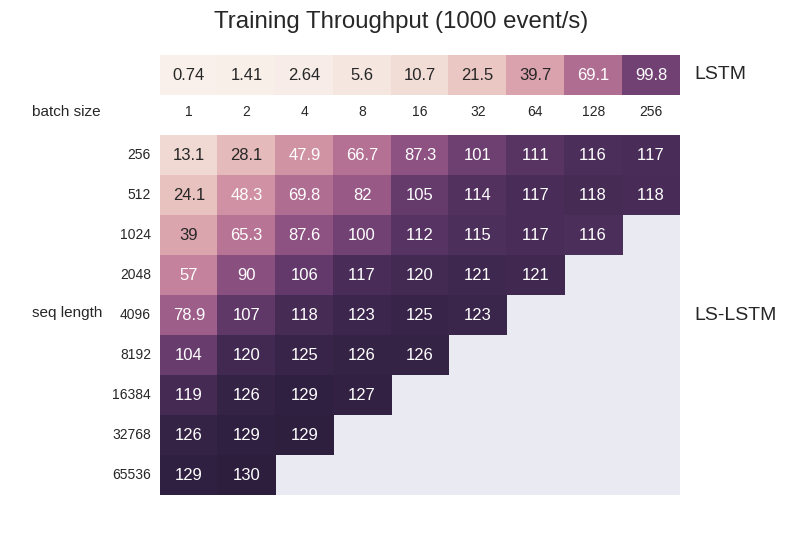
\includegraphics[width=12cm]{heatmap.png}
\caption{Throughput comparison between LSTM-256-256 with LS-LSTM-256-256. The LSTM only has a single row of data because its throughput is independent of sequence length. Entries are missing from the LS-LSTM table because there was not enough memory on the GPU to handle such large batch sizes and sequences.}
\label{fig:tp_perf}
\end{figure}

\subsection{Training performance}
The speed of neural net training is not solely determined by the training throughput but also by the frequency of optimization steps. As an example, a batch method may process inputs at the same rate as a minibatch method, but the minibatch method will generally converge much faster on large datasets. On an infinite dataset, the batch method never takes a single optimization step regardless of its throughput. With this example in mind, it is clear that achieving fast training is a balancing act between training data throughput and optimization step latency and that training performance should be evaluated with training curves and not just throughput numbers such as time per epoch.

The LSTM and LS-LSTM offer differ latency and throughput tradeoffs. LSTM throughput depends only on minibatch size but LSTM latency depends on both minibatch size and sequence length. Experiments were conducted training the LSTM models with minibatch size 256 and sequence lengths 128, 256, 512, and 1024. Figure \ref{fig:learning_curves} shows the smaller sequence lengths led to faster initial learning but inferior final performance. 

The throughput and latency of the LS-LSTM are both influenced by batch size and sequence length. Several LS-LSTMs were trained with batch size 16 and sequence length 1024. This combination was chosen because of the nearly maximum throughput, the low latency, and the ease of building a minibatch given the distribution of sequence lengths in the data set. The 234 unit LS-LSTM reaches a better training loss in roughly 4.5 hours than any of the LSTMs could reach in 18 hours. This experimental evidence indicates the LS-LSTM is as powerful of a model as the LSTM and can be trained in a fraction of the time.

\begin{figure}[t]
\centering
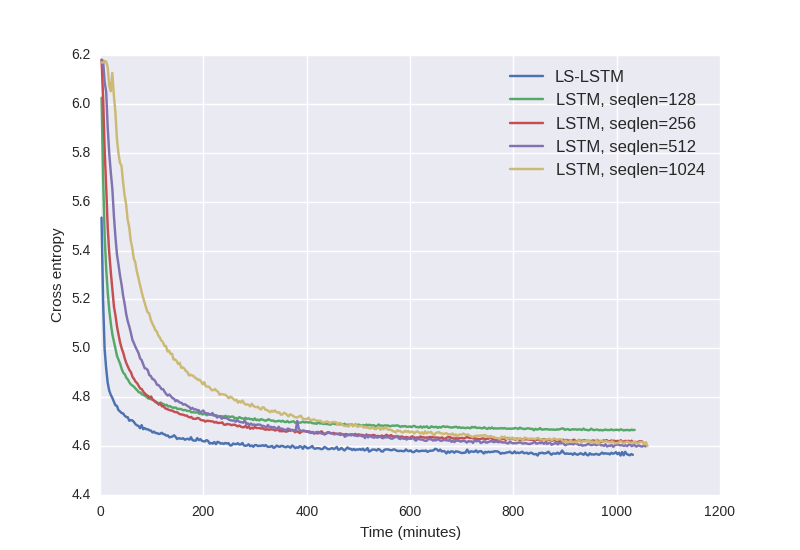
\includegraphics[width=12cm]{lc2.png}
\caption{The LSTM models had a direct relationship between sequence length and training curve: the shorter the sequence length, the faster the initial learning and
the higher the final loss. The faster initial learning is explained by the decreased
latency of optimization steps and the higher final loss is explained by the
inability to learn long dependencies. The LS-LSTM has 234 units per hidden
layer to have the same number of parameters as the 256 unit LSTMs.}
\label{fig:learning_curves}
\end{figure}

\subsection{Test performance}
\begin{table}[h]
  \caption{N-MNIST test results}
  \label{test-results}
  \centering
  \begin{tabular}{lllll}
    \toprule
    & Train Cross Entropy     & Test Cross Entropy     & Top-5 Accuracy & Top-20 Accuracy \\
    \midrule
    LS-LSTM 			&  \textbf{4.567} & 4.856           & 10.51\% & 36.70\%   \\
    LSTM, seqlen=128    & 4.664 & \textbf{4.846}  & \textbf{10.62\%} & \textbf{37.08\%}   \\
    LSTM, seqlen=256    & 4.620                & 4.906           & 10.11\% & 35.40\%   \\
    LSTM, seqlen=512    & 4.602                & 4.883           & 10.45\% & 36.32\%   \\
    LSTM, seqlen=1024   & 4.611                & 4.880           & 10.32\% & 35.92\%   \\
    \bottomrule
  \end{tabular}
\end{table}
Beyond cross entropy on train and test, we also evaluated top-$k$ accuracy for $k=5, 20$. A probability distribution is top-$k$ correct if it assigns the realized location one of the
$k$ largest probabilities. N-MNIST contains 1156 pixel positions, so top-5 and top-20 accuracy are equivalent to localizing the future to 0.43\% and 1.7\% of pixels. 

No regularization was attempted and all of the models overfit, as indicated by the best test performance from the model with the worst train performance. Table \ref{test-results} contains the full test results. Our focus was the fast training of powerful models, and we leave regularizing parallel linear recurrences and LS-RNNs to future work. Although not tested, it is possible that the LS-LSTM generalized better than the LSTMs trained on long sequences due to the much smaller minibatch size of LS-LSTM leading to a wider minima.

\section{Conclusion}
Parallel linear recurrence is an extremely powerful algorithm and the LS-LSTM is just one
of many possible models that can be built with it. Future applications of parallel linear recurrence could include sequences orders of magnitude longer than N-MNIST, the development of parallel computable differentiable memory modules, and the combination of linear recurrence with convolutional sequence models. Besides future research, existing models such as Quasi-RNNs and strongly typed RNNs that already contain linear recurrences can immediately benefit from parallel linear recurrence. This work demonstrates the LS-LSTM significantly accelerates the training of small to medium sized LSTMs. Although similar techniques have been used before, the now explicit concept of linear surrogacy provides a framework for future development and analysis of fast sequence models.

We intend to expand upon the experiments section and open-source the parallel linear recurrence kernel in the near future.

\subsubsection*{Acknowledgments}
We would like to acknowledge Kevin Bowers, Alex Meiburg, JD Co-Reyes, Carson McNeil, and several others for fruitful conversations and guidance.

\bibliography{references}

\end{document}
